% Created by tikzDevice version 0.12.6 on 2026-08-17 03:26:47
% !TEX encoding = UTF-8 Unicode
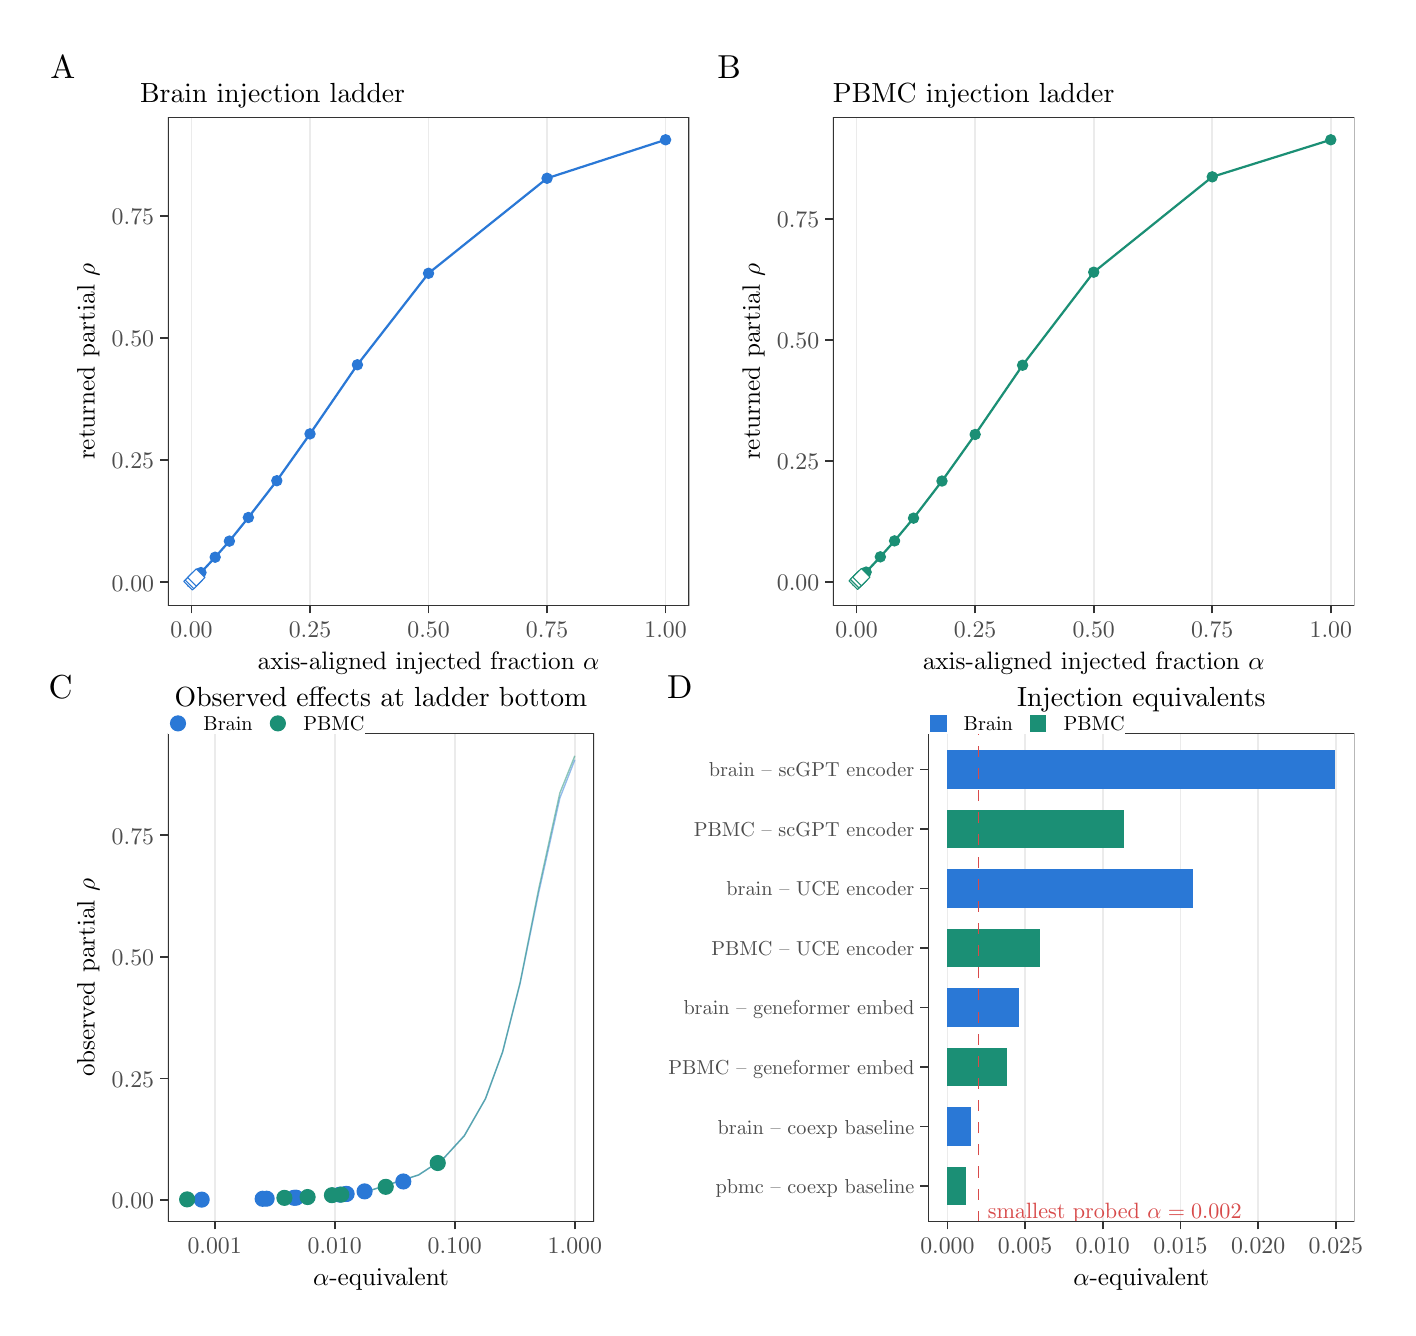
\begin{tikzpicture}[x=1pt,y=1pt]
\definecolor{fillColor}{RGB}{255,255,255}
\path[use as bounding box,fill=fillColor,fill opacity=0.00] (0,0) rectangle (491.44,462.53);
\begin{scope}
\path[clip] (  0.00,  0.00) rectangle (491.44,462.53);
\definecolor{drawColor}{RGB}{255,255,255}
\definecolor{fillColor}{RGB}{255,255,255}

\path[draw=drawColor,line width= 0.6pt,line join=round,line cap=round,fill=fillColor] ( -0.00,  0.00) rectangle (491.44,462.53);
\end{scope}
\begin{scope}
\path[clip] (  4.00,225.60) rectangle (245.08,458.53);
\definecolor{drawColor}{RGB}{255,255,255}
\definecolor{fillColor}{RGB}{255,255,255}

\path[draw=drawColor,line width= 0.6pt,line join=round,line cap=round,fill=fillColor] (  4.00,225.60) rectangle (245.08,458.53);
\end{scope}
\begin{scope}
\path[clip] (245.08,225.60) rectangle (485.44,458.53);
\definecolor{drawColor}{RGB}{255,255,255}
\definecolor{fillColor}{RGB}{255,255,255}

\path[draw=drawColor,line width= 0.6pt,line join=round,line cap=round,fill=fillColor] (245.08,225.60) rectangle (485.44,458.53);
\end{scope}
\begin{scope}
\path[clip] ( 50.62,253.62) rectangle (239.08,430.03);
\definecolor{fillColor}{RGB}{255,255,255}

\path[fill=fillColor] ( 50.62,253.62) rectangle (239.08,430.03);
\definecolor{drawColor}{gray}{0.92}

\path[draw=drawColor,line width= 0.6pt,line join=round] ( 59.19,253.62) --
	( 59.19,430.03);

\path[draw=drawColor,line width= 0.6pt,line join=round] (102.02,253.62) --
	(102.02,430.03);

\path[draw=drawColor,line width= 0.6pt,line join=round] (144.85,253.62) --
	(144.85,430.03);

\path[draw=drawColor,line width= 0.6pt,line join=round] (187.68,253.62) --
	(187.68,430.03);

\path[draw=drawColor,line width= 0.6pt,line join=round] (230.51,253.62) --
	(230.51,430.03);
\definecolor{fillColor}{RGB}{42,120,214}

\path[fill=fillColor,fill opacity=0.16] ( 59.19,262.64) --
	( 62.61,266.02) --
	( 67.75,271.59) --
	( 72.89,277.45) --
	( 79.75,286.12) --
	( 90.03,299.35) --
	(102.02,316.10) --
	(119.15,341.05) --
	(144.85,374.01) --
	(187.68,408.16) --
	(230.51,422.01) --
	(230.51,422.01) --
	(187.68,408.06) --
	(144.85,373.64) --
	(119.15,340.40) --
	(102.02,314.93) --
	( 90.03,298.40) --
	( 79.75,284.97) --
	( 72.89,276.53) --
	( 67.75,270.64) --
	( 62.61,265.19) --
	( 59.19,261.64) --
	cycle;

\path[] ( 59.19,262.64) --
	( 62.61,266.02) --
	( 67.75,271.59) --
	( 72.89,277.45) --
	( 79.75,286.12) --
	( 90.03,299.35) --
	(102.02,316.10) --
	(119.15,341.05) --
	(144.85,374.01) --
	(187.68,408.16) --
	(230.51,422.01);

\path[] (230.51,422.01) --
	(187.68,408.06) --
	(144.85,373.64) --
	(119.15,340.40) --
	(102.02,314.93) --
	( 90.03,298.40) --
	( 79.75,284.97) --
	( 72.89,276.53) --
	( 67.75,270.64) --
	( 62.61,265.19) --
	( 59.19,261.64);
\definecolor{drawColor}{RGB}{42,120,214}

\path[draw=drawColor,line width= 0.8pt,line join=round] ( 59.19,262.09) --
	( 62.61,265.63) --
	( 67.75,271.18) --
	( 72.89,276.99) --
	( 79.75,285.52) --
	( 90.03,298.82) --
	(102.02,315.74) --
	(119.15,340.72) --
	(144.85,373.77) --
	(187.68,408.11) --
	(230.51,422.01);
\definecolor{fillColor}{RGB}{42,120,214}

\path[draw=drawColor,line width= 0.4pt,line join=round,line cap=round,fill=fillColor] ( 59.19,262.09) circle (  1.86);

\path[draw=drawColor,line width= 0.4pt,line join=round,line cap=round,fill=fillColor] ( 62.61,265.63) circle (  1.86);

\path[draw=drawColor,line width= 0.4pt,line join=round,line cap=round,fill=fillColor] ( 67.75,271.18) circle (  1.86);

\path[draw=drawColor,line width= 0.4pt,line join=round,line cap=round,fill=fillColor] ( 72.89,276.99) circle (  1.86);

\path[draw=drawColor,line width= 0.4pt,line join=round,line cap=round,fill=fillColor] ( 79.75,285.52) circle (  1.86);

\path[draw=drawColor,line width= 0.4pt,line join=round,line cap=round,fill=fillColor] ( 90.03,298.82) circle (  1.86);

\path[draw=drawColor,line width= 0.4pt,line join=round,line cap=round,fill=fillColor] (102.02,315.74) circle (  1.86);

\path[draw=drawColor,line width= 0.4pt,line join=round,line cap=round,fill=fillColor] (119.15,340.72) circle (  1.86);

\path[draw=drawColor,line width= 0.4pt,line join=round,line cap=round,fill=fillColor] (144.85,373.77) circle (  1.86);

\path[draw=drawColor,line width= 0.4pt,line join=round,line cap=round,fill=fillColor] (187.68,408.11) circle (  1.86);

\path[draw=drawColor,line width= 0.4pt,line join=round,line cap=round,fill=fillColor] (230.51,422.01) circle (  1.86);
\definecolor{fillColor}{RGB}{255,255,255}

\path[draw=drawColor,line width= 0.4pt,line join=round,line cap=round,fill=fillColor] ( 59.53,259.34) --
	( 62.66,262.47) --
	( 59.53,265.60) --
	( 56.40,262.47) --
	cycle;

\path[draw=drawColor,line width= 0.4pt,line join=round,line cap=round,fill=fillColor] ( 60.04,259.77) --
	( 63.17,262.90) --
	( 60.04,266.03) --
	( 56.91,262.90) --
	cycle;

\path[draw=drawColor,line width= 0.4pt,line join=round,line cap=round,fill=fillColor] ( 60.90,260.72) --
	( 64.03,263.85) --
	( 60.90,266.98) --
	( 57.77,263.85) --
	cycle;
\definecolor{drawColor}{gray}{0.20}

\path[draw=drawColor,line width= 0.6pt,line join=round,line cap=round] ( 50.62,253.62) rectangle (239.08,430.03);
\end{scope}
\begin{scope}
\path[clip] (  0.00,  0.00) rectangle (491.44,462.53);
\definecolor{drawColor}{gray}{0.30}

\node[text=drawColor,anchor=base east,inner sep=0pt, outer sep=0pt, scale=  0.86] at ( 45.67,258.92) {0.00};

\node[text=drawColor,anchor=base east,inner sep=0pt, outer sep=0pt, scale=  0.86] at ( 45.67,303.08) {0.25};

\node[text=drawColor,anchor=base east,inner sep=0pt, outer sep=0pt, scale=  0.86] at ( 45.67,347.23) {0.50};

\node[text=drawColor,anchor=base east,inner sep=0pt, outer sep=0pt, scale=  0.86] at ( 45.67,391.38) {0.75};
\end{scope}
\begin{scope}
\path[clip] (  0.00,  0.00) rectangle (491.44,462.53);
\definecolor{drawColor}{gray}{0.20}

\path[draw=drawColor,line width= 0.6pt,line join=round] ( 47.87,262.12) --
	( 50.62,262.12);

\path[draw=drawColor,line width= 0.6pt,line join=round] ( 47.87,306.27) --
	( 50.62,306.27);

\path[draw=drawColor,line width= 0.6pt,line join=round] ( 47.87,350.42) --
	( 50.62,350.42);

\path[draw=drawColor,line width= 0.6pt,line join=round] ( 47.87,394.58) --
	( 50.62,394.58);
\end{scope}
\begin{scope}
\path[clip] (  0.00,  0.00) rectangle (491.44,462.53);
\definecolor{drawColor}{gray}{0.20}

\path[draw=drawColor,line width= 0.6pt,line join=round] ( 59.19,250.87) --
	( 59.19,253.62);

\path[draw=drawColor,line width= 0.6pt,line join=round] (102.02,250.87) --
	(102.02,253.62);

\path[draw=drawColor,line width= 0.6pt,line join=round] (144.85,250.87) --
	(144.85,253.62);

\path[draw=drawColor,line width= 0.6pt,line join=round] (187.68,250.87) --
	(187.68,253.62);

\path[draw=drawColor,line width= 0.6pt,line join=round] (230.51,250.87) --
	(230.51,253.62);
\end{scope}
\begin{scope}
\path[clip] (  0.00,  0.00) rectangle (491.44,462.53);
\definecolor{drawColor}{gray}{0.30}

\node[text=drawColor,anchor=base,inner sep=0pt, outer sep=0pt, scale=  0.86] at ( 59.19,242.28) {0.00};

\node[text=drawColor,anchor=base,inner sep=0pt, outer sep=0pt, scale=  0.86] at (102.02,242.28) {0.25};

\node[text=drawColor,anchor=base,inner sep=0pt, outer sep=0pt, scale=  0.86] at (144.85,242.28) {0.50};

\node[text=drawColor,anchor=base,inner sep=0pt, outer sep=0pt, scale=  0.86] at (187.68,242.28) {0.75};

\node[text=drawColor,anchor=base,inner sep=0pt, outer sep=0pt, scale=  0.86] at (230.51,242.28) {1.00};
\end{scope}
\begin{scope}
\path[clip] (  0.00,  0.00) rectangle (491.44,462.53);
\definecolor{drawColor}{RGB}{0,0,0}

\node[text=drawColor,anchor=base,inner sep=0pt, outer sep=0pt, scale=  0.91] at (144.85,230.75) {axis-aligned injected fraction $\alpha$};
\end{scope}
\begin{scope}
\path[clip] (  0.00,  0.00) rectangle (491.44,462.53);
\definecolor{drawColor}{RGB}{0,0,0}

\node[text=drawColor,rotate= 90.00,anchor=base,inner sep=0pt, outer sep=0pt, scale=  0.91] at ( 24.22,341.83) {returned partial $\rho$};
\end{scope}
\begin{scope}
\path[clip] (  0.00,  0.00) rectangle (491.44,462.53);
\definecolor{drawColor}{RGB}{0,0,0}

\node[text=drawColor,anchor=base west,inner sep=0pt, outer sep=0pt, scale=  1.00] at ( 40.62,435.40) {Brain injection ladder};
\end{scope}
\begin{scope}
\path[clip] (  0.00,  0.00) rectangle (491.44,462.53);
\definecolor{drawColor}{RGB}{0,0,0}

\node[text=drawColor,anchor=base,inner sep=0pt, outer sep=0pt, scale=  1.20] at ( 12.74,444.22) {A};
\end{scope}
\begin{scope}
\path[clip] (290.98,253.62) rectangle (479.44,430.03);
\definecolor{fillColor}{RGB}{255,255,255}

\path[fill=fillColor] (290.98,253.62) rectangle (479.44,430.03);
\definecolor{drawColor}{gray}{0.92}

\path[draw=drawColor,line width= 0.6pt,line join=round] (299.54,253.62) --
	(299.54,430.03);

\path[draw=drawColor,line width= 0.6pt,line join=round] (342.37,253.62) --
	(342.37,430.03);

\path[draw=drawColor,line width= 0.6pt,line join=round] (385.21,253.62) --
	(385.21,430.03);

\path[draw=drawColor,line width= 0.6pt,line join=round] (428.04,253.62) --
	(428.04,430.03);

\path[draw=drawColor,line width= 0.6pt,line join=round] (470.87,253.62) --
	(470.87,430.03);
\definecolor{fillColor}{RGB}{27,143,117}

\path[fill=fillColor,fill opacity=0.16] (299.54,262.93) --
	(302.97,266.56) --
	(308.11,271.85) --
	(313.25,277.58) --
	(320.10,285.61) --
	(330.38,299.24) --
	(342.37,315.87) --
	(359.51,340.96) --
	(385.21,374.24) --
	(428.04,408.66) --
	(470.87,422.01) --
	(470.87,422.01) --
	(428.04,408.58) --
	(385.21,374.04) --
	(359.51,340.14) --
	(342.37,315.16) --
	(330.38,298.26) --
	(320.10,284.77) --
	(313.25,276.69) --
	(308.11,270.76) --
	(302.97,265.16) --
	(299.54,261.64) --
	cycle;

\path[] (299.54,262.93) --
	(302.97,266.56) --
	(308.11,271.85) --
	(313.25,277.58) --
	(320.10,285.61) --
	(330.38,299.24) --
	(342.37,315.87) --
	(359.51,340.96) --
	(385.21,374.24) --
	(428.04,408.66) --
	(470.87,422.01);

\path[] (470.87,422.01) --
	(428.04,408.58) --
	(385.21,374.04) --
	(359.51,340.14) --
	(342.37,315.16) --
	(330.38,298.26) --
	(320.10,284.77) --
	(313.25,276.69) --
	(308.11,270.76) --
	(302.97,265.16) --
	(299.54,261.64);
\definecolor{drawColor}{RGB}{27,143,117}

\path[draw=drawColor,line width= 0.8pt,line join=round] (299.54,262.39) --
	(302.97,265.80) --
	(308.11,271.31) --
	(313.25,277.08) --
	(320.10,285.29) --
	(330.38,298.70) --
	(342.37,315.53) --
	(359.51,340.55) --
	(385.21,374.17) --
	(428.04,408.62) --
	(470.87,422.01);
\definecolor{fillColor}{RGB}{27,143,117}

\path[draw=drawColor,line width= 0.4pt,line join=round,line cap=round,fill=fillColor] (299.54,262.39) circle (  1.86);

\path[draw=drawColor,line width= 0.4pt,line join=round,line cap=round,fill=fillColor] (302.97,265.80) circle (  1.86);

\path[draw=drawColor,line width= 0.4pt,line join=round,line cap=round,fill=fillColor] (308.11,271.31) circle (  1.86);

\path[draw=drawColor,line width= 0.4pt,line join=round,line cap=round,fill=fillColor] (313.25,277.08) circle (  1.86);

\path[draw=drawColor,line width= 0.4pt,line join=round,line cap=round,fill=fillColor] (320.10,285.29) circle (  1.86);

\path[draw=drawColor,line width= 0.4pt,line join=round,line cap=round,fill=fillColor] (330.38,298.70) circle (  1.86);

\path[draw=drawColor,line width= 0.4pt,line join=round,line cap=round,fill=fillColor] (342.37,315.53) circle (  1.86);

\path[draw=drawColor,line width= 0.4pt,line join=round,line cap=round,fill=fillColor] (359.51,340.55) circle (  1.86);

\path[draw=drawColor,line width= 0.4pt,line join=round,line cap=round,fill=fillColor] (385.21,374.17) circle (  1.86);

\path[draw=drawColor,line width= 0.4pt,line join=round,line cap=round,fill=fillColor] (428.04,408.62) circle (  1.86);

\path[draw=drawColor,line width= 0.4pt,line join=round,line cap=round,fill=fillColor] (470.87,422.01) circle (  1.86);
\definecolor{fillColor}{RGB}{255,255,255}

\path[draw=drawColor,line width= 0.4pt,line join=round,line cap=round,fill=fillColor] (299.89,259.49) --
	(303.02,262.62) --
	(299.89,265.75) --
	(296.76,262.62) --
	cycle;

\path[draw=drawColor,line width= 0.4pt,line join=round,line cap=round,fill=fillColor] (300.40,260.05) --
	(303.53,263.18) --
	(300.40,266.31) --
	(297.27,263.18) --
	cycle;

\path[draw=drawColor,line width= 0.4pt,line join=round,line cap=round,fill=fillColor] (301.26,260.84) --
	(304.39,263.97) --
	(301.26,267.10) --
	(298.13,263.97) --
	cycle;
\definecolor{drawColor}{gray}{0.20}

\path[draw=drawColor,line width= 0.6pt,line join=round,line cap=round] (290.98,253.62) rectangle (479.44,430.03);
\end{scope}
\begin{scope}
\path[clip] (  0.00,  0.00) rectangle (491.44,462.53);
\definecolor{drawColor}{gray}{0.30}

\node[text=drawColor,anchor=base east,inner sep=0pt, outer sep=0pt, scale=  0.86] at (286.03,259.10) {0.00};

\node[text=drawColor,anchor=base east,inner sep=0pt, outer sep=0pt, scale=  0.86] at (286.03,302.81) {0.25};

\node[text=drawColor,anchor=base east,inner sep=0pt, outer sep=0pt, scale=  0.86] at (286.03,346.53) {0.50};

\node[text=drawColor,anchor=base east,inner sep=0pt, outer sep=0pt, scale=  0.86] at (286.03,390.24) {0.75};
\end{scope}
\begin{scope}
\path[clip] (  0.00,  0.00) rectangle (491.44,462.53);
\definecolor{drawColor}{gray}{0.20}

\path[draw=drawColor,line width= 0.6pt,line join=round] (288.23,262.30) --
	(290.98,262.30);

\path[draw=drawColor,line width= 0.6pt,line join=round] (288.23,306.01) --
	(290.98,306.01);

\path[draw=drawColor,line width= 0.6pt,line join=round] (288.23,349.72) --
	(290.98,349.72);

\path[draw=drawColor,line width= 0.6pt,line join=round] (288.23,393.43) --
	(290.98,393.43);
\end{scope}
\begin{scope}
\path[clip] (  0.00,  0.00) rectangle (491.44,462.53);
\definecolor{drawColor}{gray}{0.20}

\path[draw=drawColor,line width= 0.6pt,line join=round] (299.54,250.87) --
	(299.54,253.62);

\path[draw=drawColor,line width= 0.6pt,line join=round] (342.37,250.87) --
	(342.37,253.62);

\path[draw=drawColor,line width= 0.6pt,line join=round] (385.21,250.87) --
	(385.21,253.62);

\path[draw=drawColor,line width= 0.6pt,line join=round] (428.04,250.87) --
	(428.04,253.62);

\path[draw=drawColor,line width= 0.6pt,line join=round] (470.87,250.87) --
	(470.87,253.62);
\end{scope}
\begin{scope}
\path[clip] (  0.00,  0.00) rectangle (491.44,462.53);
\definecolor{drawColor}{gray}{0.30}

\node[text=drawColor,anchor=base,inner sep=0pt, outer sep=0pt, scale=  0.86] at (299.54,242.28) {0.00};

\node[text=drawColor,anchor=base,inner sep=0pt, outer sep=0pt, scale=  0.86] at (342.37,242.28) {0.25};

\node[text=drawColor,anchor=base,inner sep=0pt, outer sep=0pt, scale=  0.86] at (385.21,242.28) {0.50};

\node[text=drawColor,anchor=base,inner sep=0pt, outer sep=0pt, scale=  0.86] at (428.04,242.28) {0.75};

\node[text=drawColor,anchor=base,inner sep=0pt, outer sep=0pt, scale=  0.86] at (470.87,242.28) {1.00};
\end{scope}
\begin{scope}
\path[clip] (  0.00,  0.00) rectangle (491.44,462.53);
\definecolor{drawColor}{RGB}{0,0,0}

\node[text=drawColor,anchor=base,inner sep=0pt, outer sep=0pt, scale=  0.91] at (385.21,230.75) {axis-aligned injected fraction $\alpha$};
\end{scope}
\begin{scope}
\path[clip] (  0.00,  0.00) rectangle (491.44,462.53);
\definecolor{drawColor}{RGB}{0,0,0}

\node[text=drawColor,rotate= 90.00,anchor=base,inner sep=0pt, outer sep=0pt, scale=  0.91] at (264.57,341.83) {returned partial $\rho$};
\end{scope}
\begin{scope}
\path[clip] (  0.00,  0.00) rectangle (491.44,462.53);
\definecolor{drawColor}{RGB}{0,0,0}

\node[text=drawColor,anchor=base west,inner sep=0pt, outer sep=0pt, scale=  1.00] at (290.98,435.40) {PBMC injection ladder};
\end{scope}
\begin{scope}
\path[clip] (  0.00,  0.00) rectangle (491.44,462.53);
\definecolor{drawColor}{RGB}{0,0,0}

\node[text=drawColor,anchor=base,inner sep=0pt, outer sep=0pt, scale=  1.20] at (253.46,444.22) {B};
\end{scope}
\begin{scope}
\path[clip] (  4.00,  3.00) rectangle (212.72,225.60);
\definecolor{drawColor}{RGB}{255,255,255}
\definecolor{fillColor}{RGB}{255,255,255}

\path[draw=drawColor,line width= 0.6pt,line join=round,line cap=round,fill=fillColor] (  4.00,  3.00) rectangle (212.72,225.60);
\end{scope}
\begin{scope}
\path[clip] (212.72,  3.00) rectangle (485.44,225.60);
\definecolor{drawColor}{RGB}{255,255,255}
\definecolor{fillColor}{RGB}{255,255,255}

\path[draw=drawColor,line width= 0.6pt,line join=round,line cap=round,fill=fillColor] (212.72,  3.00) rectangle (485.44,225.60);
\end{scope}
\begin{scope}
\path[clip] ( 50.62, 31.02) rectangle (204.72,207.43);
\definecolor{fillColor}{RGB}{255,255,255}

\path[fill=fillColor] ( 50.62, 31.02) rectangle (204.72,207.43);
\definecolor{drawColor}{gray}{0.92}

\path[draw=drawColor,line width= 0.6pt,line join=round] ( 67.57, 31.02) --
	( 67.57,207.43);

\path[draw=drawColor,line width= 0.6pt,line join=round] (110.95, 31.02) --
	(110.95,207.43);

\path[draw=drawColor,line width= 0.6pt,line join=round] (154.33, 31.02) --
	(154.33,207.43);

\path[draw=drawColor,line width= 0.6pt,line join=round] (197.72, 31.02) --
	(197.72,207.43);
\definecolor{drawColor}{RGB}{42,120,214}

\path[draw=drawColor,draw opacity=0.50,line width= 0.5pt,line join=round] (124.01, 42.42) --
	(141.27, 47.94) --
	(150.13, 53.73) --
	(157.77, 62.21) --
	(165.41, 75.44) --
	(171.60, 92.28) --
	(177.94,117.13) --
	(184.66,150.00) --
	(192.30,184.16) --
	(197.72,197.99);
\definecolor{drawColor}{RGB}{27,143,117}

\path[draw=drawColor,draw opacity=0.50,line width= 0.5pt,line join=round] (124.01, 42.45) --
	(141.27, 47.99) --
	(150.13, 53.79) --
	(157.77, 62.03) --
	(165.41, 75.51) --
	(171.60, 92.42) --
	(177.94,117.56) --
	(184.66,151.34) --
	(192.30,185.96) --
	(197.72,199.41);
\definecolor{drawColor}{RGB}{42,120,214}
\definecolor{fillColor}{RGB}{42,120,214}

\path[draw=drawColor,line width= 0.4pt,line join=round,line cap=round,fill=fillColor] (135.74, 45.60) circle (  2.71);

\path[draw=drawColor,line width= 0.4pt,line join=round,line cap=round,fill=fillColor] ( 96.24, 39.71) circle (  2.71);

\path[draw=drawColor,line width= 0.4pt,line join=round,line cap=round,fill=fillColor] ( 62.88, 39.04) circle (  2.71);

\path[draw=drawColor,line width= 0.4pt,line join=round,line cap=round,fill=fillColor] ( 97.00, 39.74) circle (  2.71);

\path[draw=drawColor,line width= 0.4pt,line join=round,line cap=round,fill=fillColor] (115.26, 41.11) circle (  2.71);

\path[draw=drawColor,line width= 0.4pt,line join=round,line cap=round,fill=fillColor] ( 86.35, 39.38) circle (  2.71);

\path[draw=drawColor,line width= 0.4pt,line join=round,line cap=round,fill=fillColor] (112.80, 40.84) circle (  2.71);

\path[draw=drawColor,line width= 0.4pt,line join=round,line cap=round,fill=fillColor] (114.97, 41.08) circle (  2.71);

\path[draw=drawColor,line width= 0.4pt,line join=round,line cap=round,fill=fillColor] (121.74, 42.02) circle (  2.71);

\path[draw=drawColor,line width= 0.4pt,line join=round,line cap=round,fill=fillColor] ( 84.91, 39.35) circle (  2.71);
\definecolor{drawColor}{RGB}{27,143,117}
\definecolor{fillColor}{RGB}{27,143,117}

\path[draw=drawColor,line width= 0.4pt,line join=round,line cap=round,fill=fillColor] (148.18, 52.27) circle (  2.71);

\path[draw=drawColor,line width= 0.4pt,line join=round,line cap=round,fill=fillColor] ( 92.77, 39.68) circle (  2.71);

\path[draw=drawColor,line width= 0.4pt,line join=round,line cap=round,fill=fillColor] ( 57.62, 39.13) circle (  2.71);

\path[draw=drawColor,line width= 0.4pt,line join=round,line cap=round,fill=fillColor] (129.39, 43.67) circle (  2.71);

\path[draw=drawColor,line width= 0.4pt,line join=round,line cap=round,fill=fillColor] (109.94, 40.65) circle (  2.71);

\path[draw=drawColor,line width= 0.4pt,line join=round,line cap=round,fill=fillColor] (113.31, 40.86) circle (  2.71);

\path[draw=drawColor,line width= 0.4pt,line join=round,line cap=round,fill=fillColor] (101.15, 39.98) circle (  2.71);
\definecolor{drawColor}{gray}{0.20}

\path[draw=drawColor,line width= 0.6pt,line join=round,line cap=round] ( 50.62, 31.02) rectangle (204.72,207.43);
\end{scope}
\begin{scope}
\path[clip] (  0.00,  0.00) rectangle (491.44,462.53);
\definecolor{drawColor}{gray}{0.30}

\node[text=drawColor,anchor=base east,inner sep=0pt, outer sep=0pt, scale=  0.86] at ( 45.67, 35.74) {0.00};

\node[text=drawColor,anchor=base east,inner sep=0pt, outer sep=0pt, scale=  0.86] at ( 45.67, 79.66) {0.25};

\node[text=drawColor,anchor=base east,inner sep=0pt, outer sep=0pt, scale=  0.86] at ( 45.67,123.58) {0.50};

\node[text=drawColor,anchor=base east,inner sep=0pt, outer sep=0pt, scale=  0.86] at ( 45.67,167.50) {0.75};
\end{scope}
\begin{scope}
\path[clip] (  0.00,  0.00) rectangle (491.44,462.53);
\definecolor{drawColor}{gray}{0.20}

\path[draw=drawColor,line width= 0.6pt,line join=round] ( 47.87, 38.93) --
	( 50.62, 38.93);

\path[draw=drawColor,line width= 0.6pt,line join=round] ( 47.87, 82.86) --
	( 50.62, 82.86);

\path[draw=drawColor,line width= 0.6pt,line join=round] ( 47.87,126.78) --
	( 50.62,126.78);

\path[draw=drawColor,line width= 0.6pt,line join=round] ( 47.87,170.70) --
	( 50.62,170.70);
\end{scope}
\begin{scope}
\path[clip] (  0.00,  0.00) rectangle (491.44,462.53);
\definecolor{drawColor}{gray}{0.20}

\path[draw=drawColor,line width= 0.6pt,line join=round] ( 67.57, 28.27) --
	( 67.57, 31.02);

\path[draw=drawColor,line width= 0.6pt,line join=round] (110.95, 28.27) --
	(110.95, 31.02);

\path[draw=drawColor,line width= 0.6pt,line join=round] (154.33, 28.27) --
	(154.33, 31.02);

\path[draw=drawColor,line width= 0.6pt,line join=round] (197.72, 28.27) --
	(197.72, 31.02);
\end{scope}
\begin{scope}
\path[clip] (  0.00,  0.00) rectangle (491.44,462.53);
\definecolor{drawColor}{gray}{0.30}

\node[text=drawColor,anchor=base,inner sep=0pt, outer sep=0pt, scale=  0.86] at ( 67.57, 19.68) {0.001};

\node[text=drawColor,anchor=base,inner sep=0pt, outer sep=0pt, scale=  0.86] at (110.95, 19.68) {0.010};

\node[text=drawColor,anchor=base,inner sep=0pt, outer sep=0pt, scale=  0.86] at (154.33, 19.68) {0.100};

\node[text=drawColor,anchor=base,inner sep=0pt, outer sep=0pt, scale=  0.86] at (197.72, 19.68) {1.000};
\end{scope}
\begin{scope}
\path[clip] (  0.00,  0.00) rectangle (491.44,462.53);
\definecolor{drawColor}{RGB}{0,0,0}

\node[text=drawColor,anchor=base,inner sep=0pt, outer sep=0pt, scale=  0.91] at (127.67,  8.16) {$\alpha$-equivalent};
\end{scope}
\begin{scope}
\path[clip] (  0.00,  0.00) rectangle (491.44,462.53);
\definecolor{drawColor}{RGB}{0,0,0}

\node[text=drawColor,rotate= 90.00,anchor=base,inner sep=0pt, outer sep=0pt, scale=  0.91] at ( 24.22,119.23) {observed partial $\rho$};
\end{scope}
\begin{scope}
\path[clip] (  0.00,  0.00) rectangle (491.44,462.53);
\definecolor{fillColor}{RGB}{255,255,255}

\path[fill=fillColor] ( 50.62,207.43) rectangle (121.74,214.83);
\end{scope}
\begin{scope}
\path[clip] (  0.00,  0.00) rectangle (491.44,462.53);
\definecolor{fillColor}{RGB}{255,255,255}

\path[fill=fillColor] ( 50.62,207.43) rectangle ( 58.02,214.83);
\definecolor{drawColor}{RGB}{42,120,214}

\path[draw=drawColor,draw opacity=0.50,line width= 0.5pt,line join=round] ( 51.36,211.13) -- ( 57.28,211.13);
\definecolor{drawColor}{RGB}{42,120,214}
\definecolor{fillColor}{RGB}{42,120,214}

\path[draw=drawColor,line width= 0.4pt,line join=round,line cap=round,fill=fillColor] ( 54.32,211.13) circle (  2.71);
\end{scope}
\begin{scope}
\path[clip] (  0.00,  0.00) rectangle (491.44,462.53);
\definecolor{fillColor}{RGB}{255,255,255}

\path[fill=fillColor] ( 86.71,207.43) rectangle ( 94.11,214.83);
\definecolor{drawColor}{RGB}{27,143,117}

\path[draw=drawColor,draw opacity=0.50,line width= 0.5pt,line join=round] ( 87.45,211.13) -- ( 93.37,211.13);
\definecolor{drawColor}{RGB}{27,143,117}
\definecolor{fillColor}{RGB}{27,143,117}

\path[draw=drawColor,line width= 0.4pt,line join=round,line cap=round,fill=fillColor] ( 90.41,211.13) circle (  2.71);
\end{scope}
\begin{scope}
\path[clip] (  0.00,  0.00) rectangle (491.44,462.53);
\definecolor{drawColor}{RGB}{0,0,0}

\node[text=drawColor,anchor=base west,inner sep=0pt, outer sep=0pt, scale=  0.73] at ( 63.52,208.44) {Brain};
\end{scope}
\begin{scope}
\path[clip] (  0.00,  0.00) rectangle (491.44,462.53);
\definecolor{drawColor}{RGB}{0,0,0}

\node[text=drawColor,anchor=base west,inner sep=0pt, outer sep=0pt, scale=  0.73] at ( 99.61,208.44) {PBMC};
\end{scope}
\begin{scope}
\path[clip] (  0.00,  0.00) rectangle (491.44,462.53);
\definecolor{drawColor}{RGB}{0,0,0}

\node[text=drawColor,anchor=base,inner sep=0pt, outer sep=0pt, scale=  1.00] at (127.67,217.20) {Observed effects at ladder bottom};
\end{scope}
\begin{scope}
\path[clip] (  0.00,  0.00) rectangle (491.44,462.53);
\definecolor{drawColor}{RGB}{0,0,0}

\node[text=drawColor,anchor=base,inner sep=0pt, outer sep=0pt, scale=  1.20] at ( 11.93,220.16) {C};
\end{scope}
\begin{scope}
\path[clip] (325.34, 31.02) rectangle (479.44,207.43);
\definecolor{fillColor}{RGB}{255,255,255}

\path[fill=fillColor] (325.34, 31.02) rectangle (479.44,207.43);
\definecolor{drawColor}{gray}{0.92}

\path[draw=drawColor,line width= 0.6pt,line join=round] (332.34, 31.02) --
	(332.34,207.43);

\path[draw=drawColor,line width= 0.6pt,line join=round] (360.41, 31.02) --
	(360.41,207.43);

\path[draw=drawColor,line width= 0.6pt,line join=round] (388.49, 31.02) --
	(388.49,207.43);

\path[draw=drawColor,line width= 0.6pt,line join=round] (416.56, 31.02) --
	(416.56,207.43);

\path[draw=drawColor,line width= 0.6pt,line join=round] (444.64, 31.02) --
	(444.64,207.43);

\path[draw=drawColor,line width= 0.6pt,line join=round] (472.71, 31.02) --
	(472.71,207.43);
\definecolor{fillColor}{RGB}{42,120,214}

\path[fill=fillColor] (332.34,101.48) rectangle (358.06,115.46);

\path[fill=fillColor] (332.34,144.50) rectangle (359.12,158.49);

\path[fill=fillColor] (332.34,187.53) rectangle (402.92,201.51);

\path[fill=fillColor] (359.12,144.50) rectangle (421.06,158.49);

\path[fill=fillColor] (402.92,187.53) rectangle (472.43,201.51);
\definecolor{fillColor}{RGB}{27,143,117}

\path[fill=fillColor] (332.34, 79.97) rectangle (353.73, 93.95);

\path[fill=fillColor] (332.34,166.02) rectangle (395.99,180.00);

\path[fill=fillColor] (332.34,122.99) rectangle (365.73,136.97);
\definecolor{fillColor}{RGB}{42,120,214}

\path[fill=fillColor] (332.34, 58.45) rectangle (340.76, 72.44);
\definecolor{fillColor}{RGB}{27,143,117}

\path[fill=fillColor] (332.34, 36.94) rectangle (339.08, 50.92);
\definecolor{drawColor}{RGB}{216,74,74}

\path[draw=drawColor,line width= 0.6pt,dash pattern=on 4pt off 4pt ,line join=round] (343.57, 31.02) -- (343.57,207.43);

\node[text=drawColor,anchor=base west,inner sep=0pt, outer sep=0pt, scale=  0.80] at (346.94, 32.36) {smallest probed $\alpha=0.002$};
\definecolor{drawColor}{gray}{0.20}

\path[draw=drawColor,line width= 0.6pt,line join=round,line cap=round] (325.34, 31.02) rectangle (479.44,207.43);
\end{scope}
\begin{scope}
\path[clip] (  0.00,  0.00) rectangle (491.44,462.53);
\definecolor{drawColor}{gray}{0.30}

\node[text=drawColor,anchor=base east,inner sep=0pt, outer sep=0pt, scale=  0.73] at (320.39, 41.24) {pbmc -- coexp baseline};

\node[text=drawColor,anchor=base east,inner sep=0pt, outer sep=0pt, scale=  0.73] at (320.39, 62.75) {brain -- coexp baseline};

\node[text=drawColor,anchor=base east,inner sep=0pt, outer sep=0pt, scale=  0.73] at (320.39, 84.27) {PBMC -- geneformer embed};

\node[text=drawColor,anchor=base east,inner sep=0pt, outer sep=0pt, scale=  0.73] at (320.39,105.78) {brain -- geneformer embed};

\node[text=drawColor,anchor=base east,inner sep=0pt, outer sep=0pt, scale=  0.73] at (320.39,127.29) {PBMC -- UCE encoder};

\node[text=drawColor,anchor=base east,inner sep=0pt, outer sep=0pt, scale=  0.73] at (320.39,148.80) {brain -- UCE encoder};

\node[text=drawColor,anchor=base east,inner sep=0pt, outer sep=0pt, scale=  0.73] at (320.39,170.32) {PBMC -- scGPT encoder};

\node[text=drawColor,anchor=base east,inner sep=0pt, outer sep=0pt, scale=  0.73] at (320.39,191.83) {brain -- scGPT encoder};
\end{scope}
\begin{scope}
\path[clip] (  0.00,  0.00) rectangle (491.44,462.53);
\definecolor{drawColor}{gray}{0.20}

\path[draw=drawColor,line width= 0.6pt,line join=round] (322.59, 43.93) --
	(325.34, 43.93);

\path[draw=drawColor,line width= 0.6pt,line join=round] (322.59, 65.44) --
	(325.34, 65.44);

\path[draw=drawColor,line width= 0.6pt,line join=round] (322.59, 86.96) --
	(325.34, 86.96);

\path[draw=drawColor,line width= 0.6pt,line join=round] (322.59,108.47) --
	(325.34,108.47);

\path[draw=drawColor,line width= 0.6pt,line join=round] (322.59,129.98) --
	(325.34,129.98);

\path[draw=drawColor,line width= 0.6pt,line join=round] (322.59,151.50) --
	(325.34,151.50);

\path[draw=drawColor,line width= 0.6pt,line join=round] (322.59,173.01) --
	(325.34,173.01);

\path[draw=drawColor,line width= 0.6pt,line join=round] (322.59,194.52) --
	(325.34,194.52);
\end{scope}
\begin{scope}
\path[clip] (  0.00,  0.00) rectangle (491.44,462.53);
\definecolor{drawColor}{gray}{0.20}

\path[draw=drawColor,line width= 0.6pt,line join=round] (332.34, 28.27) --
	(332.34, 31.02);

\path[draw=drawColor,line width= 0.6pt,line join=round] (360.41, 28.27) --
	(360.41, 31.02);

\path[draw=drawColor,line width= 0.6pt,line join=round] (388.49, 28.27) --
	(388.49, 31.02);

\path[draw=drawColor,line width= 0.6pt,line join=round] (416.56, 28.27) --
	(416.56, 31.02);

\path[draw=drawColor,line width= 0.6pt,line join=round] (444.64, 28.27) --
	(444.64, 31.02);

\path[draw=drawColor,line width= 0.6pt,line join=round] (472.71, 28.27) --
	(472.71, 31.02);
\end{scope}
\begin{scope}
\path[clip] (  0.00,  0.00) rectangle (491.44,462.53);
\definecolor{drawColor}{gray}{0.30}

\node[text=drawColor,anchor=base,inner sep=0pt, outer sep=0pt, scale=  0.86] at (332.34, 19.68) {0.000};

\node[text=drawColor,anchor=base,inner sep=0pt, outer sep=0pt, scale=  0.86] at (360.41, 19.68) {0.005};

\node[text=drawColor,anchor=base,inner sep=0pt, outer sep=0pt, scale=  0.86] at (388.49, 19.68) {0.010};

\node[text=drawColor,anchor=base,inner sep=0pt, outer sep=0pt, scale=  0.86] at (416.56, 19.68) {0.015};

\node[text=drawColor,anchor=base,inner sep=0pt, outer sep=0pt, scale=  0.86] at (444.64, 19.68) {0.020};

\node[text=drawColor,anchor=base,inner sep=0pt, outer sep=0pt, scale=  0.86] at (472.71, 19.68) {0.025};
\end{scope}
\begin{scope}
\path[clip] (  0.00,  0.00) rectangle (491.44,462.53);
\definecolor{drawColor}{RGB}{0,0,0}

\node[text=drawColor,anchor=base,inner sep=0pt, outer sep=0pt, scale=  0.91] at (402.39,  8.16) {$\alpha$-equivalent};
\end{scope}
\begin{scope}
\path[clip] (  0.00,  0.00) rectangle (491.44,462.53);
\definecolor{fillColor}{RGB}{255,255,255}

\path[fill=fillColor] (325.34,207.43) rectangle (396.46,214.83);
\end{scope}
\begin{scope}
\path[clip] (  0.00,  0.00) rectangle (491.44,462.53);
\definecolor{fillColor}{RGB}{255,255,255}

\path[fill=fillColor] (325.34,207.43) rectangle (332.73,214.83);
\definecolor{fillColor}{RGB}{42,120,214}

\path[fill=fillColor] (326.05,208.14) rectangle (332.02,214.11);
\end{scope}
\begin{scope}
\path[clip] (  0.00,  0.00) rectangle (491.44,462.53);
\definecolor{fillColor}{RGB}{255,255,255}

\path[fill=fillColor] (361.43,207.43) rectangle (368.83,214.83);
\definecolor{fillColor}{RGB}{27,143,117}

\path[fill=fillColor] (362.14,208.14) rectangle (368.12,214.11);
\end{scope}
\begin{scope}
\path[clip] (  0.00,  0.00) rectangle (491.44,462.53);
\definecolor{drawColor}{RGB}{0,0,0}

\node[text=drawColor,anchor=base west,inner sep=0pt, outer sep=0pt, scale=  0.73] at (338.23,208.44) {Brain};
\end{scope}
\begin{scope}
\path[clip] (  0.00,  0.00) rectangle (491.44,462.53);
\definecolor{drawColor}{RGB}{0,0,0}

\node[text=drawColor,anchor=base west,inner sep=0pt, outer sep=0pt, scale=  0.73] at (374.33,208.44) {PBMC};
\end{scope}
\begin{scope}
\path[clip] (  0.00,  0.00) rectangle (491.44,462.53);
\definecolor{drawColor}{RGB}{0,0,0}

\node[text=drawColor,anchor=base,inner sep=0pt, outer sep=0pt, scale=  1.00] at (402.39,217.20) {Injection equivalents};
\end{scope}
\begin{scope}
\path[clip] (  0.00,  0.00) rectangle (491.44,462.53);
\definecolor{drawColor}{RGB}{0,0,0}

\node[text=drawColor,anchor=base,inner sep=0pt, outer sep=0pt, scale=  1.20] at (235.69,220.16) {D};
\end{scope}
\end{tikzpicture}
